\section{Towards Weakly Supervised Temporal Uncertainty Localization}
\label{sec:non_static}

Existing mechanistic approaches to hallucination detection face a recurring
tension between coverage and scalability. On one hand, traditional probing
classifiers \citep{azaria2023, orgad2024} operate on a single
layer--token position, inspecting only a small slice of the activation
tensor $A$. Predictive signals elsewhere in $A$ are ignored, and the
optimal probing position varies across samples, datasets, and LLMs --
often requiring an external search procedure to identify, which can entail
multiple expensive LLM queries \citep{orgad2024}. On the other hand,
methods that process the full activation tensor capture these distributed
signals but are not well suited to real-time, long-form generation: some
must collapse the token axis into a fixed-size representation, so the
signal dilutes as responses grow longer, while others remain accurate at
long context but are too costly to run as each token is produced. Even
when a full-tensor method does scale, it typically emits a single
sequence-level score and cannot indicate \emph{where} in the response the
suspicious activations lie. For long answers, where most of the generated
text is typically correct and only a few regions are problematic, a
sequence-level score is both harder to interpret and less actionable for
downstream verification or correction.

\begin{figure}[t]
\centering
\fbox{\begin{minipage}{0.95\linewidth}\centering\vspace{4em}\textit{[Figure 2: Test AUC heatmaps across layer--token combinations --- placeholder]}\vspace{4em}\end{minipage}}
\caption{Test AUC heatmaps across layer--token combinations; best layer-token combinations are boxed.}
\label{fig:heatmaps}
\end{figure}


\paragraph{Signals are distributed and LLM-specific.} We first provide
empirical support for the limitations of static probing. Inspired by the
analyses of \citet{orgad2024} on Mistral-7B-Instruct-v0.2
\citep{albertqjiang2023} (Mis-7B), we train distinct logistic regression
classifiers for each layer--token combination and construct ROC-AUC
heatmaps to visualize the presence and localization of hallucination
signals. We conduct this analysis across three LLMs and five datasets.
Since responses vary in length, we restrict tokens to
$\mathcal{N} := \{0, 1, 2, -3, -2, -1\}$, namely the first and last three
positions in each response. Heatmaps are presented in
Figure~\ref{fig:heatmaps} for Mis-7B, Llama-3-8B-Instruct
\citep{touvron2023} (LlaMa-8B), and Qwen2.5-7B-Instruct \citep{yang2024}
(Qwen-7B) on the Movies dataset \citep{orgad2024} (full set in
Appendix~\ref{app:extended}). Predictive signals are spread across many
layer--token combinations, but the most informative positions vary
substantially across LLMs: signals concentrate around the middle layers
for Mis-7B and LlaMa-8B, while for Qwen-7B they sit in the final layers.
Concretely, the best probing position for Mis-7B, $(14, 0)$, transfers
poorly: it is $\approx 7\%$ AUC below the per-LLM optimum on both LlaMa-8B
and Qwen-7B. No fixed layer--token slice suffices across LLMs, motivating
models that consume the full activation tensor.

\begin{figure}[t]
\centering
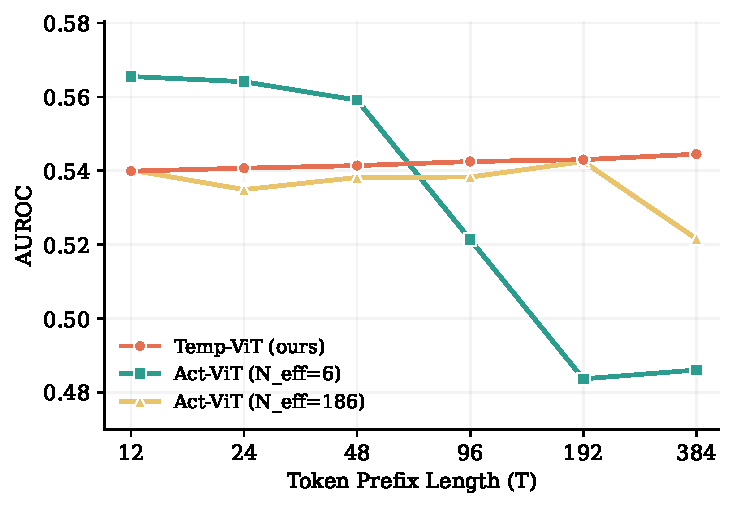
\includegraphics[width=0.95\linewidth]{figs/fig_perf_by_length.pdf}
\caption{Per-token AUROC on the LongFact prefix-truncation test as the
generated-token prefix length $T$ fed to each model grows. ACT-ViT
with its default short pooled token axis (\emph{Act-ViT, N\textsubscript{eff}=6})
peaks at short prefixes but collapses past $T = 48$ and falls below
chance for $T \in \{192, 384\}$ as the pooling compresses an
increasing number of token positions into the same fixed-size image.
Raising the pooled axis (\emph{Act-ViT, N\textsubscript{eff}=186})
partially rescues long prefixes but does not match Temp-ViT's flat
profile, which is per-token by construction. This illustrates the
long-form weakness of activation-tensor methods that pool the token
axis into a fixed-size representation.}
\label{fig:perf_by_length}
\end{figure}

\begin{figure}[t]
\centering
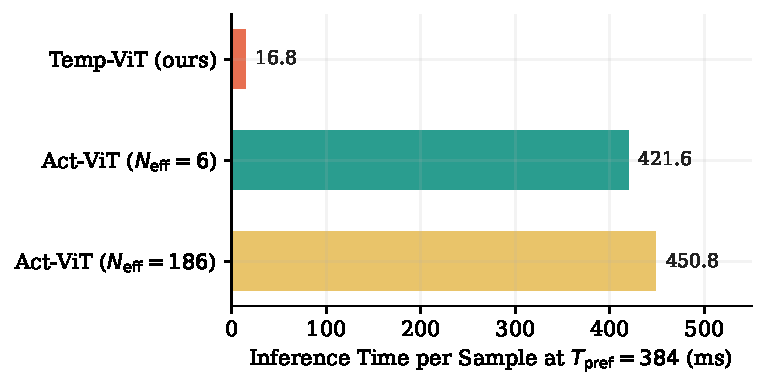
\includegraphics[width=0.95\linewidth]{figs/fig_inference_time.pdf}
\caption{Wall-clock time to score every token of one $T = 384$-token
LongFact passage on a single H200, batch~1, FP32. ACT-ViT emits one
scalar per call, so labelling every token requires $T$ sequential
forwards; per-call latency is small but the total scales linearly with
the response length, even when the post-pool ViT input is widened to
recover long-range accuracy (\emph{N\textsubscript{eff}=186}).
Temp-ViT produces the full per-token logit vector in a single forward
pass and is roughly $25\times$ faster on this passage, illustrating
the real-time-cost weakness of activation-tensor methods that need one
call per generated token.}
\label{fig:inference_time}
\end{figure}


\paragraph{Tensor methods scale poorly with response length.} Models
that already consume the full activation tensor must contend with the
second tension noted above: long-form responses either dilute their
signal or blow up their inference cost. We show both effects
empirically. Figure~\ref{fig:perf_by_length} reports per-token AUROC
on the LongFact prefix-truncation test as the generated-token prefix
length $T$ grows from 12 to 384. ACT-ViT with its default short
pooled token axis peaks at very short prefixes but collapses past
$T = 48$, falling below chance for $T \in \{192, 384\}$ as a growing
number of token positions is squeezed through the same fixed-size
pooled image; widening the pooled axis from 6 to 186 patches up the
long-prefix collapse but does not recover the short-prefix peak and
leaves a $4\times$ wider AUROC spread than a per-token model on the
same data. Figure~\ref{fig:inference_time} reports the corresponding
wall-clock cost of producing predictions at every token of one
$T = 384$ passage on a single H200: ACT-ViT emits one scalar per call,
so labelling every token requires $T$ sequential forwards and the
total latency scales linearly with the response length, even when the
post-pool input is widened. A per-token model that produces the
entire logit vector in a single forward is $\approx 25\times$ faster
on this passage, and -- crucially -- does not require choosing between
short-prefix accuracy and long-prefix stability. Together, these two
results motivate models whose architecture is per-token by
construction rather than pooled-then-classified.

\paragraph{From sequence-level detection to localization.} Even given a
model that processes the full $A$, a single sequence-level score is
insufficient for long-form generation. A long response may interleave
mostly correct text with a few uncertain spans; a sequence-level prediction
can flag the response as risky, but cannot tell a user -- or a downstream
verifier -- which spans to scrutinize. We therefore aim to additionally
produce per-window uncertainty scores $\{\hat{p}^{(t)}\}_{t=1}^{T}$ that
localize the generated-token regions whose hidden-state activations most
contribute to the sequence-level prediction.

\paragraph{The weak-supervision challenge.} Localization is challenging
because hallucination labels are typically available only at the response
level. A natural workaround is to extract atomic claims from the response,
verify each claim against ground truth, and broadcast the verification
result to every token in the claim's span. Token-level labels obtained
this way are noisy in two complementary senses. First, the span is more
granular than the response but still coarser than a token: it typically
contains tokens that are not themselves hallucinated, so inheriting the
span's label overestimates the support of the signal. Second, the
hidden-state patterns that drive a hallucination may appear before the
false claim is generated -- e.g., during the model's processing of the
question or earlier context -- so claim-aligned spans can also miss part
of the relevant signal. We therefore treat span labels as a coarse
auxiliary supervision signal rather than as ground-truth token labels,
and rely on weak supervision to localize \emph{within} the span.

\paragraph{Weakly supervised temporal localization.} ACT-ViT shows that
the layer--token plane of $A$ has spatial structure amenable to visual
encoders, but framing $A$ as a single image fits the activation tensor
poorly when the number of generated tokens varies from a handful to
thousands: any fixed-size image must pool or crop along the token axis.
We instead frame $A$ as a \emph{video} over the token axis and borrow
weakly supervised temporal localization (WSTL) from video understanding
\citep{pilhyeonlee2021}. In WSTL for action recognition, the model is
told only that an action occurs somewhere in a video and must learn to
identify the consecutive frames that span it. By analogy, each generated
token plays the role of a ``frame'': a frame's ``height'' is the layer
axis, its ``width'' is a single token, and its ``channels'' are the
hidden dimension; a \emph{window} aggregates the activations of $W$
consecutive tokens. Just as a video model identifies the windows of
frames spanning an action without frame-level labels, our model
identifies the windows of tokens whose activation patterns carry
uncertainty without window-level labels.

\paragraph{Three-stage training.} Learning sequence-level uncertainty
quantification \emph{and} window-level localization jointly under weak
supervision is a difficult optimization: the model must simultaneously
discover which activation patterns indicate uncertainty and which windows
contain them, which is prone to overfitting and noisy predictions in the
limited-data regime typical of hallucination annotation. To make this
tractable, we decompose training into three stages, each focused on one
task. In Stage~1, we train an encoder on full activation tensors with
sequence-level labels, so it learns activation patterns predictive of
uncertainty. In Stage~2, we freeze the encoder and train a temporal head
over per-window encodings on per-atom segments, focusing on aggregating
information across tokens and localizing uncertain regions within a
single atom. The temporal head emits a per-window logit $\hat{p}^{(t)}$,
and a top-$k$ multiple-instance learning rule averages the $k$ most
uncertain windows into a sequence-level logit against which the head is
supervised; mean-of-top-$k$ is more stable than alternative aggregations,
especially for long sequences. We use Mamba \citep{albertgu2024} for the
temporal head because it processes long sequences efficiently, making the
method viable for real-time long-form generation.

Stages~1 and~2 alone, however, never expose the temporal head to the
context in which it is deployed: passages contain many atoms at once,
and a head trained only on isolated atom segments has no incentive to
discriminate the uncertain atoms from the confident ones that sit
beside them. Stage~3 closes this gap by fine-tuning the head, still
under the same frozen encoder, on whole passages with the per-atom
auxiliary span labels introduced above. The head's per-token logits are
smoothed along the token axis and then aggregated within each atom span
into a per-atom logit, against which we apply a per-atom binary
cross-entropy. The result is a temporal head that ranks uncertainty
\emph{across} the atoms inside a passage rather than scoring each atom
in isolation; concrete forms of the smoothing and segment aggregation
are detailed in the next section, where we describe the encoder
(Stage~1), the temporal head (Stage~2), and the passage-level refinement
(Stage~3) in turn.
